\fbox{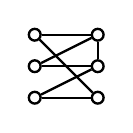
\begin{tikzpicture}[myv/.style={circle, draw, inner sep=1.5pt,line width=0.3mm}]
  \node (z) at (0,0) {};

  \node[myv] (a) at (-0.4,0.4) {};
  \node[myv] (b) at (0.4,0.4) {};
  \node[myv] (c) at (-0.4,0) {};
  \node[myv] (d) at (0.4,0) {};
  \node[myv] (e) at (-0.4,-0.4) {};
  \node[myv] (f) at (0.4,-0.4) {};
 

  
  \draw [line width=0.3mm](a) -- (b);
  \draw [line width=0.3mm](b) -- (c);
  \draw [line width=0.3mm](c) -- (d);
  \draw [line width=0.3mm](d) -- (e);
  \draw [line width=0.3mm](e) -- (f);
  \draw [line width=0.3mm](f) -- (a);

  \draw [line width=0.3mm] (b) -- (d);
\end{tikzpicture}}